\documentclass[12pt]{{memoir}}
\usepackage{graphicx}
\usepackage[overlay]{textpos}
\usepackage[hidelinks,pdfusetitle]{hyperref}
\usepackage{xfrac}
\usepackage[paperwidth=7.5in,paperheight=10.0in,top=.5in,bottom=.5in,left=.25in,right=.25in]{geometry}

\newcommand\Hline{%
\hline\raisebox{0pt}[1.125em]{}}


\interfootnotelinepenalty=10000
\begin{document}
\title{Retro 6k Emulator User's Guide}
\author{Maggie\,David P.\,K. Haynes}
\pagestyle{empty}
\begin{center}
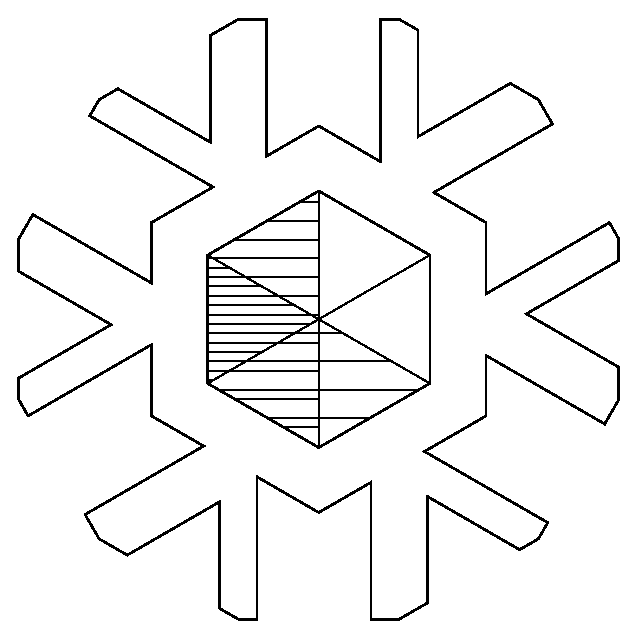
\includegraphics{../common-src/logolineart}

\vspace{\stretch{.25}}
{\sffamily\bfseries\Huge{}Retro 6k\\Fantasy Computer\\Entertainment System

\vspace{\stretch{1}}
Emulator User's Guide\par}
\vspace*{\stretch{1}}
{\sffamily\bfseries\large\theauthor\par}
\end{center}
\vspace*{\stretch{3}}
\cleartoverso
\vspace*{\stretch{2}}
\begin{center}
\noindent{}Here's where I\\
write a personal note...\par
\end{center}

\vspace*{\stretch{3}}
\cleartorecto
\tableofcontents*
\clearpage
\pagestyle{headings}

\vspace*{3in}
\section*{Conventions Used In This Document}

Nothing established yet.

\chapter{Emulator Startup}

When the Retro 6k emulator starts, the first thing it does is ask which cartridge to ``insert''. If you press \textsf{Esc}, the cartridge selection closes and the system boots without a cartridge inserted. If you do select a cartridge, the emulator may then ask you to choose which ``instance'' of the selected cartridge to load; the physical equivalent is which of multiple copies of a cartridge are inserted into the machine. This will only happen if the selected cartridge is designed to store data persistently. The process is described in greater detail in chapter \ref{ch:loadcartridge} on page \ref{ch:loadcartridge}. Following the selection of a cartridge and possibly an instance file, the system boots with the selected cartridge inserted.

\cleartoverso
\pagestyle{empty}
\vspace*{\stretch{1}}

\noindent\thetitle\hfill\textcopyright2019--20 \theauthor

\end{document}
